% $Header: /cvsroot/latex-beamer/latex-beamer/solutions/generic-talks/generic-ornate-15min-45min.en.tex,v 1.5 2007/01/28 20:48:23 tantau Exp $

\documentclass{beamer}
%\documentclass[mathsherif]{beamer}

% This file is a solution template for:

% - Giving a talk on some subject.
% - The talk is between 15min and 45min long.
% - Style is ornate.



% Copyright 2004 by Till Tantau <tantau@users.sourceforge.net>.
%
% In principle, this file can be redistributed and/or modified under
% the terms of the GNU Public License, version 2.
%
% However, this file is supposed to be a template to be modified
% for your own needs. For this reason, if you use this file as a
% template and not specifically distribute it as part of a another
% package/program, I grant the extra permission to freely copy and
% modify this file as you see fit and even to delete this copyright
% notice.


\mode<presentation>
{
\usecolortheme[RGB={89,165,140}]{structure}

  \usetheme{Warsaw}
\setbeamercolor*{palette quaternary}{fg=white,bg=structure!40!black}


% o Singapore
% \setbeamercolor{normal text}{bg=blue!10} % para azul, la oscuridad del color se regula cambiando (!20)
% \beamertemplateshadingbackground{yellow!50}{magenta!50} % degradado de amarillo a magenta
  % or ...
% \setbeamertemplate{navigation symbols}{} quitar l\'{\i}nea de s\'{\i}mbolos esquina inferior derecha -in\'{u}tiles
  \setbeamercovered{transparent}
  % or whatever (possibly just delete it)
}


\usepackage[spanish]{babel}
% or whatever

\usepackage[latin1]{inputenc}
% or whatever

\usepackage{times}
\usepackage[T1]{fontenc}
\usepackage{lmodern}

%\usepackage{lucidaso}
%\usepackage[small]{eulervm}

% Paquetes de David
\usepackage{verbatim}
\usepackage{listings}
\usepackage{color}
\usepackage{etoolbox}
\usepackage{xstring}
\usepackage{../gsi-parametros}
 
\definecolor{dkgreen}{rgb}{0,0.6,0}
\definecolor{gray}{rgb}{0.5,0.5,0.5}
\definecolor{mauve}{rgb}{0.58,0,0.82}
  
\lstset{ %
  language=Java,                % the language of the code
  basicstyle=\footnotesize,           % the size of the fonts that are used for the code
  %numbers=left,                   % where to put the line-numbers
  numberstyle=\tiny\color{gray},  % the style that is used for the line-numbers
  numbersep=5pt,                  % how far the line-numbers are from the code
%  backgroundcolor=\color{white},      % choose the background color. You must add \usepackage{color}
  showspaces=false,               % show spaces adding particular underscores
  showstringspaces=false,         % underline spaces within strings
  showtabs=false,                 % show tabs within strings adding particular underscores
  %frame=single,                   % adds a frame around the code
  rulecolor=\color{black},        % if not set, the frame-color may be changed on line-breaks within not-black text (e.g. commens (green here))
  tabsize=2,                      % sets default tabsize to 2 spaces
  captionpos=b,                   % sets the caption-position to bottom
  breaklines=true,                % sets automatic line breaking
  breakatwhitespace=false,        % sets if automatic breaks should only happen at whitespace
  %title=\lstname,                   % show the filename of files included with \lstinputlisting;
  keywordstyle=\color{blue},          % keyword style
  commentstyle=\color{dkgreen},       % comment style
  stringstyle=\color{mauve},         % string literal style
  escapeinside={\%*}{*)},            % if you want to add a comment within your code
  morekeywords={*,...}               % if you want to add more keywords to the set
}


% Or whatever. Note that the encoding and the font should match. If T1
% does not look nice, try deleting the line with the fontenc.

% para Singapore
%\setbeamertemplate{footline}{%
%\leavevmode%
%\hbox{%
%\begin{beamercolorbox}[wd=.333333\paperwidth,ht=2.25ex,dp=1ex,center]{author in head/foot}%
%\usebeamerfont{author in head/foot}\insertshortauthor
%\end{beamercolorbox}%
%\begin{beamercolorbox}[wd=.333333\paperwidth,ht=2.25ex,dp=1ex,center]{title in head/foot}%
%\usebeamerfont{title in head/foot}\insertshorttitle
%\end{beamercolorbox}%
%\begin{beamercolorbox}[wd=.333333\paperwidth,ht=2.25ex,dp=1ex,right]{date in head/foot}%
%\usebeamerfont{date in head/foot}\insertshortdate{}\hspace*{2em}
%\insertframenumber{} / \inserttotalframenumber\hspace*{2ex}
%\end{beamercolorbox}}%
%\vskip0pt%
%}
%
% para Warsaw
\newcommand*\oldmacro{}%
\let\oldmacro\insertshorttitle%
\renewcommand*\insertshorttitle{%
  \oldmacro\hfill%
  \insertframenumber\,/\,\inserttotalframenumber}

%\renewcommand*{\appendixname}{Referencias}


\title[Getting started] % (optional, use only with long paper titles)
{Getting started}

%\subtitle
%{Presentation Subtitle} % (optional)

\author[\asignatura] % (optional, use only with lots of authors)
{\autor}
% - Use the \inst{?} command only if the authors have different
%   affiliation.

\institute[Universidad de Alcal\'{a}] % (optional, but mostly needed)
{
  %\inst{1}%
  \textcolor{structure} {\emph{\textbf{Departamento de Autom\'{a}tica}}}\\
  Universidad de Alcal\'{a}

% - Use the \inst command only if there are several affiliations.
% - Keep it simple, no one is interested in your street address.

%\date[Short Occasion] % (optional)
%{Date / Occasion}

\vspace*{0.5cm}
\includegraphics[height=0.8cm]{comun/uah}
}
\date{}



%logos s\'{o}lo en title
\titlegraphic{
  \includegraphics[scale=0.45]{comun/dpto}
  \hfill
 % \includegraphics[scale=0.35]{gso1}
 % \hfill
  \includegraphics[scale=0.20]{comun/gso1}
}

% logos tal cual: salen en todos los frames...
%\pgfdeclareimage[height=0.4cm]{left-logo}{gso1}
%\pgfdeclareimage[height=0.4cm]{right-logo}{gso1}
%\logo{\pgfuseimage{right-logo}}


%\setbeamertemplate{sidebar left}
%{
%\logo{\pgfuseimage{left-logo}}
%\vfill%
%\rlap{\hskip0.1cm\insertlogo}%
%\vskip15pt%
%}

\subject{Talks}
% This is only inserted into the PDF information catalog. Can be left
% out.



% If you have a file called "university-logo-filename.xxx", where xxx
% is a graphic format that can be processed by latex or pdflatex,
% resp., then you can add a logo as follows:


% marca de agua de una imagen

\usebackgroundtemplate{\includegraphics[width=\paperwidth]{comun/marcadeagua}}


%% QUITAR LOS PARES %% DE LAS L\'{I}NEAS DE \AtBeginSubsection PARA QUE SE GENERE LA NAVEGACI\'{O}N EN LA SUBSECCIONES
%%\AtBeginSubsection[]
%% {
%%     \begin{frame}{\'{I}ndice}
%  \small
%  \tableofcontents[currentsection,hideothersubsections]
%  \normalsize
% \end{frame}

%%    \small
%%    \tableofcontents[currentsection,currentsubsection]
     % \tableofcontents[pausesections]
%%   \end{frame}
%%}

%% QUITAR LOS PARES %% DE LAS L\'{I}NEAS DE \AtBeginSubsection PARA QUE SE GENERE LA NAVEGACI\'{O}N EN LA SUBSECCIONES
%%\AtBeginSection[]
%% {
%%     \begin{frame}{\'{I}ndice}
%  \small
%  \tableofcontents[currentsection,hideothersubsections]
%  \normalsize
% \end{frame}

%%    \small
%%    \tableofcontents[currentsection]
     % \tableofcontents[pausesections]
%%   \end{frame}
%%}

% If you wish to uncover everything in a step-wise fashion, uncomment
% the following command:

%\beamerdefaultoverlayspecification{<+->}


\begin{document}

\begin{frame}[plain]
  \titlepage
\end{frame}

\begin{frame}[plain]{}
   \begin{block}{Objectives}
      \begin{enumerate}
         \item Understand the concept of programming language
         \item Introduce interpreted and compiled languages
         \item Describe the Java Virtual Machine
         \item First contact with Java code
      \end{enumerate} 
   \end{block}

   \begin{block}{Bibliography}
      \begin{enumerate}
          \item The Java\textsuperscript{TM} Tutorials. Oracle. \href{https://docs.oracle.com/javase/tutorial/}{(Link)}
      \end{enumerate} 
   \end{block}


\end{frame}

\begin{frame}[shrink]{Table of Contents}
 \frametitle{Table of Contents}
 \tableofcontents

 % no me vale: deja descolgado el cap\'{\i}tulo 4
 % \frame[allowframebreaks]%
 %    {\frametitle{\'{I}ndice}\tableofcontents[part=4]}
  % You might wish to add the option [pausesections]
\end{frame}


% Since this a solution template for a generic talk, very little can
% be said about how it should be structured. However, the talk length
% of between 15min and 45min and the theme suggest that you stick to
% the following rules:

% - Exactly two or three sections (other than the summary).
% - At *most* three subsections per section.
% - Talk about 30s to 2min per frame. So there should be between about
%   15 and 30 frames, all told.

\section{Programming languages}

\begin{frame}[plain]{Programming languages (I)}
	\textbf{Programming language}: A formal language designed to communicate instructions to a machine

	\vspace{-0.2cm}
   	 	\begin{figure}[t]
		\begin{center}
		    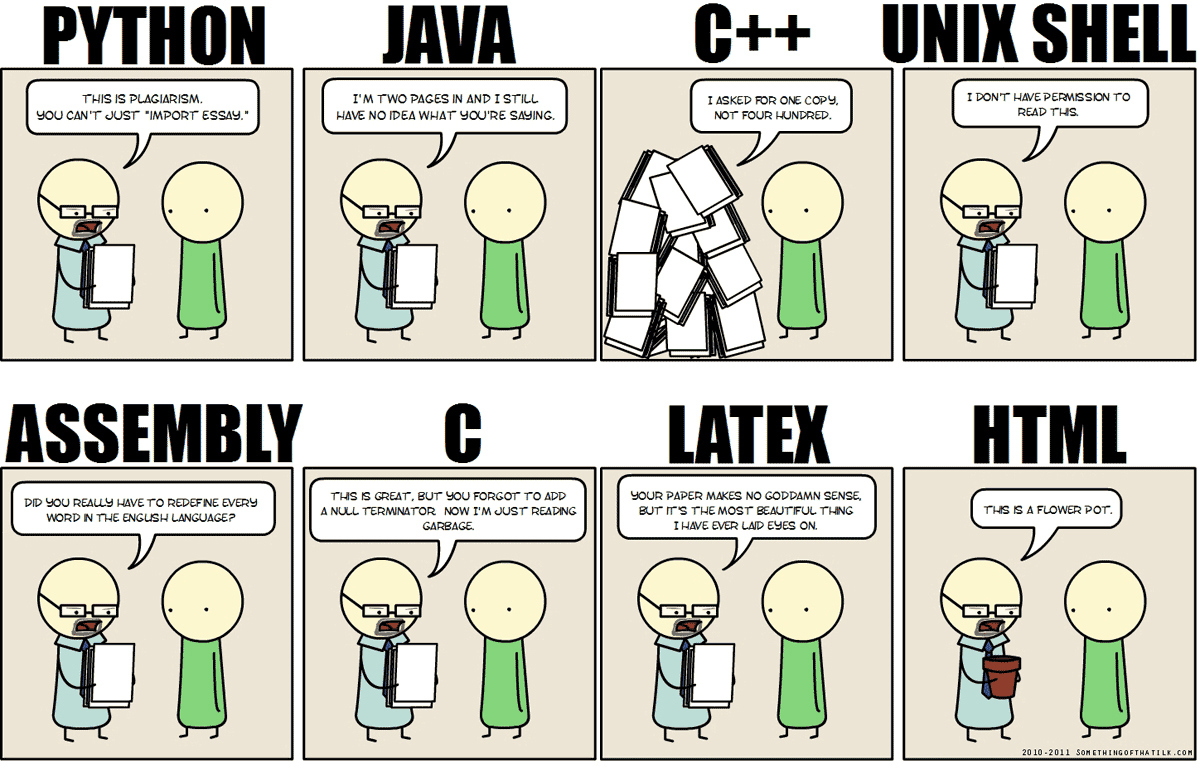
\includegraphics[width=\linewidth]{figs/lenguajes.jpg}
		\end{center}
   	 	\end{figure}

\end{frame}

\begin{frame}{Programming languages (II)}
	Languages types
	\begin{itemize}
		\item \textit{Compiled}: C, C++, Pascal, ...
		\item \textit{Interpreted} (\alert{scripts}): Python, Perl, PHP, ...
 	\end{itemize}

	\begin{columns}
 	   \column{.50\textwidth}
		\begin{tabular}{|l|l|l|}
		\hline
		      		& Compiled 	& Interpreted  \\\hline
		Speed 		& Fast 	 	& Slow 		\\
		Development	& Slow 	 	& Fast 		\\
		Abstraction & Low/High	& High 		\\
		Flexibility & Low		& High 		\\
		Project size& Large		& Small 	\\\hline
		\end{tabular}
 	   \column{.50\textwidth}
		\begin{figure}[t]
		\begin{center}
		    
\includegraphics[width=0.7\linewidth]{figs/wordmap.png}
		\end{center}
   	 	\end{figure}
\end{columns}
\end{frame}

\section{Overview of Java}

\subsection[Why Java?]{Why Java?}
\begin{frame}{Overview of Java}{Why Java? (I)}
	\begin{itemize}
	\item Widely used in the industry
		\begin{itemize}
		\item Good point in your CV!
		\end{itemize}
	\item Large number of domains
		\begin{itemize}
		\item Desktop applications, servers, embedded systems, tablets, mobiles, ...
		\item Videogames industry shifts to wider range of platforms
		\item Java videogames for mobile platforms
		\end{itemize}
	\item Clean and elegant object-oriented language
	\item High level (do more with less code)
	\item Syntax similar to other languages
	\item Availability of videogames source code
  	\end{itemize}
\end{frame}

\begin{frame}{Overview of Java}{Why Java? (II)}
    \begin{columns}
 	   \column{.50\textwidth}
	   \begin{block}{Advantages}
  		\begin{itemize}
		\item Device independent
		\item Safety
		\item Java standards
		\item Object-oriented
		\item Many applications
  		\end{itemize}
		\end{block}
 	   \column{.50\textwidth}
		\begin{block}{Disadvantages}
		\begin{itemize}
		\item Slower execution
		\item Difficult device specific features
		\item JVM availability
		\item Huge ecosystem
  		\end{itemize}
		\end{block}
	\end{columns}
\end{frame}


\subsection[About the Java technology]{About the Java technology}
\begin{frame}{Overview of Java}{About the Java technology}
    \begin{columns}
 	   \column{.70\textwidth}
  		  \begin{itemize}
			\item Java was created by Sun Microsystems
		   	\begin{itemize}
				\item Now Java belongs to Oracle
		  	\end{itemize}

			\item History
		   	\begin{itemize}
				\item 1.0 (1996), 1.1 (1997), 1.2 (1998), 1.3 (2000), 1.4 (2002)
				\item 5 (2004), 6 (2006), 7 (2011), 8 (2014)
		  	\end{itemize}
		\item Java is a programming language and a platform
	    	\begin{itemize}
			\item Programming language: Like C or C++
			\item Platform: Where programs run, including hardware and operating system
	    	\end{itemize}
		  	\end{itemize}
   	 \column{.30\textwidth}
   	 	\begin{figure}[t]
		\begin{center}
		    
\includegraphics[width=0.6\linewidth]{figs/java}\\
			\bigskip
		    
\includegraphics[width=0.6\linewidth]{figs/Sun}\\
			\bigskip
		    
\includegraphics[width=0.6\linewidth]{figs/oracle}
		\end{center}
   	 	\end{figure}
    \end{columns}

\end{frame}

\subsection[Java as programming language]{Java as programming language}
\begin{frame}{Overview of Java}{Java as programming language (I)}
	\begin{center}
	The standard way\\
	\bigskip
	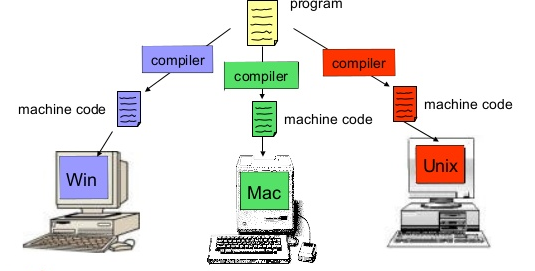
\includegraphics[width=0.8\linewidth]{figs/compilacion}\\
	\scriptsize{\href{http://es.slideshare.net/darokoblog/an-introduction-to-java-programming-language-forbeginnersjava-programming-tutorials}{(Source)}}
	\end{center}
\end{frame}

\begin{frame}{Overview of Java}{Java as programming language (II)}
	\begin{center}
	The Java way: \textit{Write once, run anywhere}\\
	\smallskip
	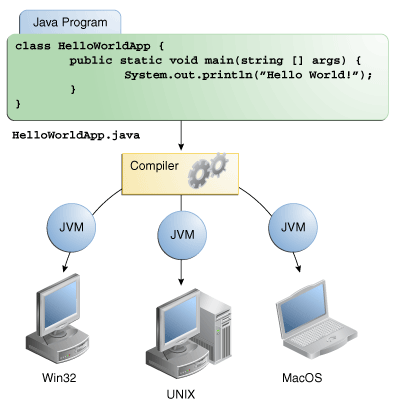
\includegraphics[width=0.5\linewidth]{figs/helloWorld}\\
	\scriptsize{\href{http://docs.oracle.com/javase/tutorial/getStarted/intro/definition.html}{(Source)}}
	\end{center}
\end{frame}

\begin{frame}{Overview of Java}{Java as programming language (III)}
	\begin{center}
	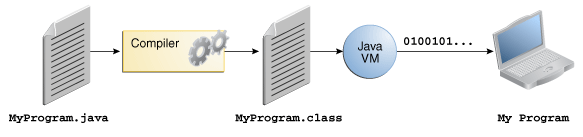
\includegraphics[width=\linewidth]{figs/getStarted-compiler}\\
	\scriptsize{\href{http://docs.oracle.com/javase/tutorial/getStarted/intro/definition.html}{(Source)}}
	\end{center}
	\bigskip

	\normalsize{\textbf{*.java:} Source code file}\\
	\normalsize{\textbf{*.class:} Bytecode file}\\
	\normalsize{\textbf{Bytecode:} Machine language of the Java Virtual Machine (JVM)}
\end{frame}
\subsection[Java as platform]{Java as platform}
\begin{frame}{Overview of Java}{Java as platform}
	\begin{itemize}
	\item A platform is all the required infraestructure to run a program
	\item Usually, hardware (CPU) + software (OS)
		\begin{itemize}
		\item In Java all the platform uses to be software
		\end{itemize}
	\item Two components: JVM (\textit{Java Virtual Machine}) and API (\textit{Application Programming Interface})
	\end{itemize}
	\centering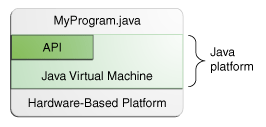
\includegraphics[width=0.5\linewidth]{figs/getStarted-jvm}\\
\end{frame}

\subsection[Acronyms]{Acronyms}
\begin{frame}{Overview of Java}{Acronyms}
	JSE: Java Standard Edition (Java Virtual Machine, JVM)\\
	JDK: Java Developer Kit (Compiler + JVM)\\
	J2EE: Java Enterprise Edition\\
	J2ME (now Java ME): Java Micro Edition\\
	Others: AWT, Swing, Ajax, EJB, HPJ, JAX, JDBC, JSP, Servlet, SAX, JDOM, ...
\end{frame}

\section[Hello world!]{Hello world!}
\begin{frame}{Hello World!}{Hello world! (I)}
	\vspace{-0.2cm}
	\begin{block}{HelloWorld.java}
		\lstinputlisting{code/HelloWorld.java}
	\end{block}

	Procedure:
	\begin{enumerate}
		\item Compile: \texttt{javac HelloWorld.java}
		\item Run: \texttt{java HelloWorld}
	\end{enumerate}
\end{frame}

\begin{frame}{Hello World!}{Hello world! (II)}
	\begin{itemize}
		\item Java is an evolution of C: Almost same syntaxis
     	\item Entry point in \texttt{main()}
		\item \texttt{System.out.println()} prints a string
		\item // and /* ... */ are comments
		\item /** ... */ is a \alert{javadoc} comment
		\item Java ignores the end of line
	    	\begin{itemize}
		 	\item `;' marks the end of instruction
 		 	\end{itemize}
		\item Keyword \texttt{class} begins the class definition
	    	\begin{itemize}
		 	\item Class name and file name \textit{must} be equal!
 		 	\end{itemize}
	\end{itemize}
\end{frame}

\section[Example]{Example}
\begin{frame}{Example}
	\vspace{-0.2cm}
	\begin{block}{Hello.java}
		\lstinputlisting{code/Hello.java}
	\end{block}

	Procedure:
	\begin{enumerate}
		\item Compile: \texttt{javac Hello.java}
		\item Run: \texttt{java Hello}
	\end{enumerate}
\end{frame}

\begin{frame}{Example}{Questions}
	\begin{enumerate}
		\item How can you compile and run the program?
		\item How would you join the two last lines?
		\item Change the program to show the number of years to 100
		\item Change the program to read and show weight (float number)
	\end{enumerate}
\end{frame}



\end{document}
